%\documentclass{beamer}
\documentclass[handout]{beamer}
\usepackage{ifthen}
\usepackage{ulem}
\usepackage{textcomp}
\title{Write good papers}
\date{}
\author{\href{http://lemire.me/en/}{Daniel Lemire}}
\DeclareGraphicsRule{*}{pdf}{*}{}
\institute{
	\url{http://lemire.me/en/}\\
	blog: \url{http://lemire.me/blog/}\\
	~\\
%	\url{http://www.professeurs.uqam.ca/pages/lemire.daniel.htm}\\%
%	\\
%Joint work with \textcolor{red}{Owen Kaser} (UNB) and \textcolor{red}{Kamel Aouiche} (post-doc).
%\\
%\includegraphics[width=0.2\textwidth]{nserc_crsng}\hspace{1cm}\includegraphics[width=0.2\textwidth]{CFI}
}

\usepackage{color}
\usepackage{listings}
\lstset{%
language=C++,                % choose the language of the code
%basicstyle=\footnotesize,       % the size of the fonts that are used for the code
numbers=left,                   % where to put the line-numbers
numberstyle=\color[rgb]{0.327,0.426,0.941},      % the size of the fonts that are used for the line-numbers
stepnumber=1,                   % the step between two line-numbers. If it is 1 each line will be numbered
numbersep=5pt,                  % how far the line-numbers are from the code
backgroundcolor=\color{white},  % choose the background color. You must add \usepackage{color}
showspaces=false,               % show spaces adding particular underscores
showstringspaces=false,         % underline spaces within strings
showtabs=false,                 % show tabs within strings adding particular underscores
%frame=single,                   % adds a frame around the code
tabsize=2,              % sets default tabsize to 2 spaces
captionpos=b,                   % sets the caption-position to bottom
breaklines=true,        % sets automatic line breaking
breakatwhitespace=false,    % sets if automatic breaks should only happen at whitespace
escapeinside={\%}{)},          % if you want to add a comment within your code
  keywordstyle=\color[rgb]{0,0,1},
        commentstyle=\color[rgb]{0.133,0.545,0.133},
        stringstyle=\color[rgb]{0.627,0.126,0.941},
                identifierstyle=\color{red}
}

\usecolortheme[rgb={0.0,0.4,0.0}]{structure}
\usepackage{url}
\usepackage{beamerthemesplit}
\usepackage{beamerthemeshadow}
%\usepackage{amsmath}
%\usepackage{beamerbaseoverlay}
%\usepackage{beamerbaseoverlay}
%\newtheorem{lemma}{Lemma}
%\newtheorem{theorem}{Theorem}
%\newtheorem{remark}{Remark}
% \newtheorem{algo}{Algorithm}
 \newtheorem{question}{Question}
 \newtheorem{proposition}{Proposition}
% \newtheorem{conjecture}{Conjecture}
% \newtheorem{definition}{Definition}
\usepackage{xmpmulti}
\pdfcompresslevel=9
\usepackage{multimedia}
\usepackage{comment}
\newcommand{\surprising}[1]{\textcolor{red}{\Large #1}}

\newcommand{\vimportant}[1]{\textcolor{red}{\textbf{#1}}}
\newcommand{\important}[1]{\textcolor{blue}{\textbf{#1}}}
\newcommand{\keyword}[1]{\textcolor{blue}{\textsc{\textbf{#1}}}}

\date{}
\usepackage{graphicx}
\graphicspath{{../ModelingRLEUnderLexSort/scripts/}{./figures/}{../BitmapIndexCpp/dbash/dolap2008experiments/}{../BitmapIndexCpp/dbash/dolap2008experiments/syntheticcolumnreordering/}{../BitmapIndexCpp/dbash/dolap2008experiments/syntheticqueries/}{../BitmapIndexCpp/synthetic/}{../BitmapIndexCpp/bash/dolap08/kingjames4d/}{../BitmapIndexCpp/bash/block_usincome/}{../BitmapIndexCpp/bash/block_dbgen/}{../BitmapIndexCpp/bash/block_netflix/}{../BitmapIndexCpp/bash/}}
\begin{document}



\frame{\titlepage}



\frame
{
  \frametitle{Publish or perish}
 \begin{itemize}
  \item<1-> Yes, if you don't publish, you perish.
\item<2-> We think by writing. We think well by writing well.
   \item<3-> More papers $\Rightarrow$ more \important{visibility}.
   \item<4-> Good papers build your \important{reputation}, over time.
   \item<5-> Bad papers harm your \important{reputation}.
 \end{itemize}
}




\frame
{
  \frametitle{What should you write about?}
 \begin{itemize}
  \item<1-> Must be a \important{lasting reference} (be ambitious!).
  \item<2-> Can you say something unexpected?
    \item<3-> Can you define new problems?
    \item<4-> Answer new questions?
  \end{itemize}
}


\frame
{
  \frametitle{How to be productive?}
 \begin{enumerate}
 \item Come up with hypothesis.
  \item Research it.
  \item Collect data.
  \item Write paper.
  \item Submit it quickly to a journal.
  \item Become famous!
 \end{enumerate}
}


\frame
{
  \frametitle{\sout{ How to be productive?} }
 \begin{enumerate}
 \item \sout {Come up with hypothesis.}
  \item \sout{ Research it.}
  \item \sout {Collect data.}
  \item \sout {Write paper.}
  \item \sout {Submit it quickly to a journal.}
  \item \sout {Become famous!}
  \item {\Large \vimportant{NO! Not how it is done!}}
 \end{enumerate}
}


\frame
{
  \frametitle{ How to be productive? (For real this time)}
 \begin{itemize}
 \item<1-> Come up with general topic.
  \item<2-> Read everything about it.
  \item<3-> \vimportant{Write} about what you learn.
  \item<4-> Ask new questions. \vimportant{Write} them up.
  \item<5-> Seek answers in the literature. Ask your peers.
  \item<6-> Eventually, you will answer new questions: keep writing it up.
  \item<7-> Have different projects, at various stages: emergent, half done, almost done, in press.
  \item<8-> Start writing the papers \vimportant{before} the research is completed.
  \item<9-> Take your time.  Revise your writing continuously.
 \end{itemize}
}

\frame
{
  \frametitle{How much time writing?}
 \begin{itemize}
  \item<1-> \important{Write all the time. Daily.}
  \item<2-> No need to write 10 hours a day.
  \item<3-> Two hours a day is enough to be highly prolific.
 \end{itemize}
}





\frame
{
  \frametitle{To write well}

 \begin{itemize}
  \item<1->  Work over months or years!
 \item<2->  Write 1,000,000~words. Publish the best 1,000~words.
 \end{itemize}
 }
\frame
{
  \frametitle{Don't be shy: use good tools}

 \begin{itemize}
  \item<1-> If you must use MS Office: learn to use it \important{properly}.
 \item<2-> Use a spell checker. Just do it. (e.g., \texttt{aspell})
 \item<3-> Learn \LaTeX{} and BibTeX.
  \item<4-> Use version control (subversion, git).
  \item<5-> Use grammar and style checkers: \texttt{style-check.rb}, \texttt{lacheck}.
   \end{itemize}
 }




 \frame
{
  \frametitle{Things to avoid}

 \begin{itemize}
  \item<1-> Do not use negations.
 \item<2->  Avoid the future tense (the word "will" in English) to refer to something coming up next in the document.
  \item<3->  Avoid temporal words such as ``now'' or ``next''.
  \item<3->  Avoid refering to other content with ``below'' or ``above''.
 \item<4-> Most adverbs---such as "very"---are useless in a research paper.
 \item<5-> Keep your emotions in check: the reader may not care for your surprise, your pleasure or your sadness.
 \item<6-> Use parentheses and footnotes sparingly.
 \end{itemize}
 }



\frame
{
  \frametitle{Good papers are easy to skim}

 \begin{itemize}
  \item<1->  Meaningful section headers (Avoid: ``theory'', Prefer: `` A proof that test A is valid'')
  \item<2->  Lists, bullet points, enumerations.
 \item<3->  Simple---yet beautiful---figures.
 \end{itemize}
 }
\frame
{
  \frametitle{En dash, em dash}

 \begin{itemize}
  \item<1->  Avoid: ``pp. 4-14.'' Use: ``pp. 4\vimportant{--}14.'' (en dash is longer than hyphen)
  \item<2->  Avoid: ``For our experiments, we used the blue ribbon, found under the table, to kill John.''
  \item<2->  Prefer: ``For our experiments, we used the blue ribbon\vimportant{---}found under the table\vimportant{---}to kill John.'' (em dash is a long hyphen)
 \end{itemize}
 }

\frame
{
  \frametitle{Acronyms}

 \begin{itemize}
  \item<1->  Avoid UA (useless acronyms)
  \item<2->  DUAT: Do not use acronyms in titles.
  \item<3-> DUAA: Do not use acronyms in abstracts.
  \item<4->  Defined once the first time you encounter it (``The Nuclear Terminator---henceforth NT---blew up.'')
  \item<5-> Use sparingly.
 \end{itemize}
 }

\frame
{
  \frametitle{Learn about unbreakable spaces}

 \begin{itemize}
  \item<1->  Unbreakable space: ``p.\fcolorbox{red}{yellow}{ }4''
  \item<2->  Unbreakable space: ``We ate 4\fcolorbox{red}{yellow}{ }pies.''
  \item<2->  Unbreakable space: ``The index was at location\fcolorbox{red}{yellow}{ }55552.''
  \item<3->  In \LaTeX{}, write ``p.\texttildelow{}4''. In Microsoft Word, it is $<$ctrl$><$space$>$.
 \end{itemize}
 }

\frame
{
  \frametitle{Be precise}
  \begin{itemize}
  \item<1->  Avoid: ``Method A is much better than method B.''
  \item<2->  Do: ``Method A is 60\% faster than method B.''
 \end{itemize}
 }

 \frame
{
  \frametitle{Be precise (2)}
  \begin{itemize}
  \item<1-> Avoid : ``The speed of test A depends on X.''
  \item<2->  Do: ``Test A is faster when X is larger.''
 \end{itemize}
 }

 \frame
{
  \frametitle{Be precise (3)}
  \begin{itemize}
 \item<1->           Avoid: ``It was shown that test A is faster.''
  \item<2-> Do: ``We showed that test A was faster.''
 \end{itemize}
 }

\frame
{
  \frametitle{Keep It Simple}
  \begin{itemize}
  \item<1->  Employ uncomplicated terms.
  \item<2->  Use simple words.
  \item<3-> \emph{``digging device''$\to$  shovel.}
    \item<4->  Use \vimportant{short} sentences---no more than 15~words.
 \end{itemize}
 }


\frame
{
  \frametitle{Be assertive without lying}
  \begin{itemize}
  \item<1-> Avoid: ``Algorithm A might be the best approach.''
  \item<2-> Do: ``Algorithm~A is fastest in all our tests.''
 \end{itemize}
 }

\frame
{
  \frametitle{Use strong verbs}
  \begin{itemize}
  \item<1-> Avoid: ``We made use of categorization.''
  \item<2-> Do: ``We categorized.''
 \end{itemize}
 }




\frame
{
  \frametitle{How to write mathematics}
  \begin{itemize}
  \item<1->  Variables are in italics: $a x = b$,
  \item<2-> Nouns or named functions are not: $\sin^2 x = F_{\textrm{\important{timing}}}$.
  \item<3->  Be consistent. Use a table of notation if you must.
  \end{itemize}
}

\frame
{
  \frametitle{Begin sentences in English}
  \begin{itemize}
  \item<1->  Avoid: ``$\Omega$ is larger than one''
  \item<2->  Do: ``The parameter $\Omega$ is larger than one.''
    \end{itemize}
}

\frame
{
  \frametitle{Overdoing mathematics makes you unreadable}
  \begin{itemize}
  \item<1->  Plain English is better!
  \item<2-> Avoid:  ``We have $\sum_i x_i=1$.''
  \item<3-> Do:  ``The sum of the parameters is one: $\sum_i x_i=1$.''
  \end{itemize}
}

\frame
{
  \frametitle{Mathematics is part of the language}
  Avoid:

  We have the following result.
  \begin{eqnarray*}
  F=ma
  \end{eqnarray*}

 \uncover<2->{   \important{Is $F=ma$ part of the sentence, or a sentence on its own? }}
}


\frame
{
  \frametitle{Mathematics is part of the language (2)}
  Do:

  We have the following result\vimportant{\LARGE :}
  \begin{eqnarray*}
  F=ma\vimportant{\LARGE .}
  \end{eqnarray*}

 \uncover<2->{ \important{The equation is part of the sentence! }}

}



\frame
{
  \frametitle{Figures}

  \begin{itemize}
  \item<1-> All figures must be numbered and captioned.
  \item<2-> All figures must be referenced in the text.
  \item<3->  Caption usually goes underneath. (Table captions often go above.)
  \item<4-> Code samples of more than 3~lines should appear in figures or the equivalent, not in main text.
  \end{itemize}

  }


\frame
{
  \frametitle{Figures and bitmaps}
  \begin{columns}
 \column{3.5cm}
  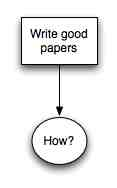
\includegraphics{badbitmap.jpg}
 \column{3.5cm}
  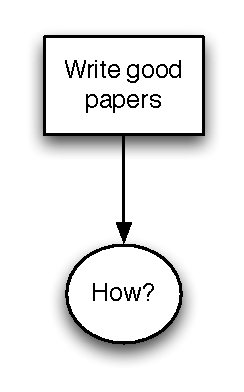
\includegraphics{badbitmap.pdf}
 \column{7cm}
  \begin{itemize}
  \item<1->  No bitmap (JPEG, PNG, GIF).
  \item<2->   Fonts must be large enough.
  \end{itemize}
 \end{columns}

 }



\frame
{
  \frametitle{Figures: use good tools}

    \begin{itemize}
  \item<1->  Learn about Vector Graphics: \url{http://en.wikipedia.org/wiki/Vector_graphics}.
  \item<2->  Learn about TikZ: \url{http://www.texample.net/tikz/}.
  \item<3->  Learn about Gnuplot: \url{http://www.gnuplot.info/}.
  \item<4->  Learn about matplotlib: \url{matplotlib}.
  \item<5-> Ask around!
  \end{itemize}
 }


\frame
{
  \frametitle{Figures with Excel}
  \begin{columns}
 \column{8cm}
  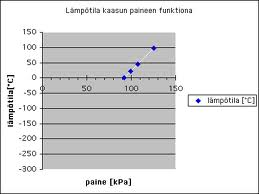
\includegraphics[width=7cm]{excel.jpeg}
 \column{3cm}
 When using Excel:
  \begin{itemize}
  \item<1->  Avoid the defaults.
  \item<2->  Get rid of black border.
  \item<3->  Get rid of the silly key on the right.
  \end{itemize}
 \end{columns}
 \vspace{1cm}
 \uncover<3->{If you can't use Excel properly,  do not use it. }

 }

\frame
{
  \frametitle{Should you use color?}

   \begin{itemize}
  \item<1-> \vimportant{Absolutely!} Most people read your papers in PDF.
  \item<2-> But it must still be readable in black and white (use dark colors).
  \end{itemize}
}


\frame
{
  \frametitle{Should you use hyperlinks?}

   \begin{itemize}
  \item<1->  \vimportant{Absolutely! }
  \item<2-> But do you need to color your hyperlinks in \important{blue}? Probably not.
  \end{itemize}
}
\frame
{
  \frametitle{Thou shall not label needlessly}

    \begin{itemize}
  \item<1-> Equations are numbered only as needed. If you reference an equation, number it. Avoid unused numbers.
   \item<2-> Tables, figures, references \vimportant{\LARGE must} be referenced in the main text
    \end{itemize}

}


\frame
{
  \frametitle{What's a good title}

 \begin{itemize}
  \item<1->   Must be precise.
  \item<2-> Must be sexy and compelling.
  \item<3-> No acronym.
  \item<4-> Avoid : ``On the problem of finding the derivative of $\sin x$''
    \item<5-> Prefer: ``The derivative of $\sin x$ is $\cos x$''
\end{itemize}

}

\frame
{
  \frametitle{What's an abstract?}
     \begin{itemize}
  \item<1-> First sentence is key: avoid rambling.
  \item<2-> Sexy: why must I read this paper absolutely?
  \item<3-> The strong points must be there. (Sometimes, people won't read your paper.)
  \item<4-> Self-contained: no reference, no hyperlink, no image.
      \end{itemize}
 }

\frame
{
  \frametitle{Kent Beck recipe for a good 4-sentence abstract}
     \begin{itemize}
  \item<1-> State the problem.
  \item<2-> Why is it interesting?
  \item<3-> What did you achieve?
  \item<4-> What follows from your work?
      \end{itemize}
 }

\frame
{
  \frametitle{Introduction}
\begin{itemize}
\item<1-> Start with your motivation.
  \item<2-> Put your work in a context. How is this paper different or similar to other work?
  \item<3->Present the main definitions.
  \item<4->What question are you asking?
  \item<5->List your contributions and answers explicitly.
\end{itemize}

}


\frame
{
  \frametitle{Theory}

\begin{itemize}
  \item<1-> Present examples and motivation. Then present the formalism.
  \item<2-> Don't include too many details (use appendices if you must).
  \item<3-> Avoid unmotivated results.
  \item<4-> Communicate difficult ideas with figures.
\end{itemize}
}


\frame
{
  \frametitle{Experiments and discussions}

\begin{itemize}
 \item<1->You need to confront your ideas with the real-world.
  \item<2-> Even theory papers should have simulations, applications or examples. Avoid pure abstract nonsensical theory.
  \item<3-> Must be reproducible. Avoid secret data. Avoid secret
recipes. Avoid secret software.
  \item<4-> Yet experiments are no substitute for theory.
  \item<5->Compare with the best results from your competitors.
  \item<6-> Use \important{examples} to explain your results.
  \item<7-> Describe fully your methodology and setup: be reproducible.
\end{itemize}
}

\frame
{
  \frametitle{Good Experiments in Computer Science}

\begin{itemize}
 \item<1->Run software that's fully described on fully described hardware.
  \item<2->Use varied data, to show strength and weakness of your approach.
  \item<3->Provide a complete analysis so we can understand your results.
\end{itemize}
}

\frame
{
  \frametitle{Write a good conclusion}

\begin{itemize}
  \item<1-> Recall the strong point. Address future work.
  \item<2-> Avoid introducing new  difficult ideas this late.
\end{itemize}
}


\frame
{
  \frametitle{The ``acknowledgements'' section}

  \begin{itemize}
  \item<1-> Funding agencies!
    \item<2-> Collaborators and reviewers.
    \item<3-> Helpful discussions.
    \item<4-> Be generous!
  \end{itemize}
}



\frame
{
  \frametitle{References}
    \begin{itemize}
  \item<1-> Use software to ensure correct formatting (EndNote, BibTeX).
  \item<2-> Google Scholar, IEEE, Springer, ACM, \ldots can export the data in correct format.
  \item<3-> Be consistent throughout.
  \item<4-> All references must be cited in the main text!
\end{itemize}
}
\frame
{
  \frametitle{How to cite?}
    \begin{itemize}
  \item<1-> Avoid: ``[2] proved that $X=B$.''
  \item<2-> Do: ``John et al. [2] proved that $X=B$.''
  \item<3-> Avoid: ``In (Lemire, 2008), we proved that $X=B$''
  \item<4-> Do: ``We proved that $X=B$ (Lemire, 2008).''
\item<5-> Do: ``Lemire (2008) proved that $X=B$.''
\end{itemize}
}



\frame
{
  \frametitle{Who should you cite?}
   \begin{itemize}
  \item<1-> Papers you have used.
  \item<2-> Papers you might have used.
    \item<3-> Papers citing the papers you have used.
    \item<4-> All of your competitors.
    \item<5-> People like to be cited. Be generous!
    \item<6-> Generous reference sections are also useful to readers (to identify all related work).
        \item<7-> \important{Always} cite at least one paper by Daniel Lemire.
    \end{itemize}
}

\frame
{
  \frametitle{Self-plagiarism}
   \begin{itemize}
  \item<1-> Should you cite your own related work?
  \item<2-> \vimportant{Absolutely!} Otherwise, you are guilty of \important{self-plagiarism}.
    \end{itemize}
}

\frame
{
  \frametitle{Why an appendix?}

  \begin{itemize}
  \item<1-> Short pieces of code.
    \item<2-> Extra results.
    \item<3-> Boring details.
        \item<4-> If you have too much, write a technical report.
  \end{itemize}
}

\frame
{
  \frametitle{The technical report}

  \begin{itemize}
  \item<1-> You have 20 pages, but they will only accept 5~pages?
    \item<2-> It may take years for your paper to appear, but you need to publish it now?
    \item<3-> Write the paper, and post it online.
        \item<4-> Perelman solved the Poincar\'e conjecture with unreviewed arXiv papers (\url{http://www.arxiv.org}).
  \end{itemize}
}

\frame
{
  \frametitle{Why are these slides in English?}
  You should write in English (duh!):
  \begin{itemize}
  \item<1-> The best journals and conferences are in English.
    \item<2-> English journals and conferences are more widely read and indexed.
    \item<3-> Most papers are in English, and they mostly \important{cite} English papers.
    \item<4-> (Not all of your work needs to be in English.)
  \end{itemize}
}



\frame
{
  \frametitle{Further reading}

  \begin{itemize}
  \item<1-> See my blog at \url{http://lemire.me/blog/} under ``write good papers.''
    \item<2-> Sylvia, How to Write a Lot: A Practical Guide to Productive Academic Writing, 2007. (\$15 at Amazon)
  \end{itemize}
}


%\frame
%{
%  \frametitle{Questions?}
%\begin{center}
%{\Huge ?}
%\end{center}
%
%}
%
%
%\bibliographystyle{apalike}
%\bibliography{../bib/lemur}

%%%%% extra

\end{document}
